\documentclass{beamer}
\usepackage[utf8]{inputenc}
\usepackage[T1]{fontenc}
\usepackage{lmodern}
\usepackage{graphicx}
\usepackage{booktabs}
\usepackage{amsmath}

\usetheme{Madrid}
\usecolortheme{default}

\title{Control PID del Sistema del Péndulo Invertido}
\subtitle{Diseño por Asignación de Polos y Validación Experimental}
\author{Lucas Gaggino}
\institute{Facultad de Ingeniería - UBA \\ Control Adaptativo 86.20}


\begin{document}

\begin{frame}
\titlepage
\end{frame}

\section{El Sistema y el Controlador}

\begin{frame}{Sistema del Péndulo Invertido}
\begin{block}{Ecuación No Lineal}
La dinámica del sistema se describe por:
\[
(M + m) \ddot{x} = F - m l \ddot{\theta} \cos\theta + m l \dot{\theta}^2 \sin\theta
\]

\[
m l \ddot{\theta} \cos\theta + m l \dot{\theta}^2 \sin\theta + m g \sin\theta = 0
\]
\end{block}

\begin{block}{Modelo Linealizado}
Aplicando linealización alrededor de $\theta = 0$:
\[
\ddot{\theta} = A_\theta \theta + B_\theta F
\]
donde $A_\theta = 15.79$ (inestable), $B_\theta = 1.46$
\end{block}
\end{frame}

\begin{frame}{Parámetros del Sistema}
\begin{block}{Valores Numéricos}
\begin{itemize}
\item Masa del carro: $M = 1.0$ kg
\item Masa del péndulo: $m = 0.1$ kg
\item Longitud del péndulo: $l = 0.5$ m
\item Gravedad: $g = 9.81$ m/s²
\end{itemize}
\end{block}

\begin{block}{Función de Transferencia Continua}
\[
G(s) = \frac{B_\theta}{s^2 - A_\theta} = \frac{1.46}{s^2 - 15.79}
\]
\end{block}

\begin{block}{Discretización}
Sistema discretizado con $T_s = 0.02$ s:
\[
G(z) = \frac{0.000293}{z^2 - 2.006z + 1.000}
\]
\end{block}
\end{frame}

\section{Diseño del Controlador PID}

\begin{frame}{Método de Diseño: Asignación de Polos}
\begin{block}{Enfoque Analítico}
El diseño del controlador PID se realizó mediante asignación de polos, especificando la dinámica deseada del sistema en lazo cerrado.
\end{block}

\begin{block}{Polinomio Característico Deseado}
Para un sistema de tercer orden (PID + planta de segundo orden):
\[
s^3 + a s^2 + b s + c = 0
\]

Polos deseados: $s = -3, -3, -10$
\end{block}
\end{frame}

\begin{frame}{Implementación del Método de Asignación de Polos}
\begin{block}{Ecuación Característica}
Para el sistema en lazo cerrado con controlador PID:
\[
C(s) = K_p + \frac{K_i}{s} + K_d s
\]

El polinomio característico resulta:
\[
s^3 + K_d B_\theta s^2 + (K_p B_\theta - A_\theta) s + K_i B_\theta = 0
\]
\end{block}

\begin{block}{Sistema de Ecuaciones}
\[
\begin{cases}
K_d B_\theta = a \\
K_p B_\theta - A_\theta = b \\
K_i B_\theta = c
\end{cases}
\]
\end{block}
\end{frame}

\begin{frame}{Cálculo de las Ganancias PID}
\begin{block}{Coeficientes del Polinomio Deseado}
Polos: $s = -3, -3, -10$
\[
\begin{aligned}
s^3 + 16s^2 + 69s + 90 &= (s+3)(s+3)(s+10) \\
&= s^3 + 16s^2 + 69s + 90
\end{aligned}
\]
\end{block}

\begin{block}{Solución del Sistema}
\[
\begin{cases}
K_d \cdot 1.46 &= 16 \\
K_p \cdot 1.46 - 15.79 &= 69 \\
K_i \cdot 1.46 &= 90
\end{cases}
\]

\[
\begin{cases}
K_d &= 10.96 \\
K_p &= 57.94 \\
K_i &= 61.64
\end{cases}
\]
\end{block}
\end{frame}

\begin{frame}{Controlador PID Implementado}
\begin{block}{Estructura del Controlador}
Controlador PID discreto implementado:
\[
u[k] = K_p e[k] + K_i \sum_{i=0}^{k} e[i] + K_d (e[k] - e[k-1])
\]

\begin{itemize}
\item $K_p = 57.94$, $K_i = 61.64$, $K_d = 10.96$
\item Tiempo de muestreo: $T_s = 0.02$ s
\item Saturación: $\pm 500$ unidades
\end{itemize}
\end{block}


\end{frame}

\section{Resultados Experimentales}

\begin{frame}{Simulaciones Realizadas}
\begin{center}
\begin{tabular}{l|c|c}
\textbf{Condición} & \textbf{Tipo} & \textbf{Parámetros} \\
\hline
Condición inicial & $\theta(0) = 0.1$ rad & Sin perturbaciones \\
Perturbación sinusoidal & $A = 0.005$ rad & $f = 0.5$ Hz \\
Perturbación escalón & $A = 0.01$ rad & $t = 5-7$ s \\
Ruido de medición & $\sigma = 0.005$ rad & Gaussiano blanco \\
\hline
\end{tabular}
\end{center}
\end{frame}

\begin{frame}{Respuesta del Sistema Controlado}
\begin{center}
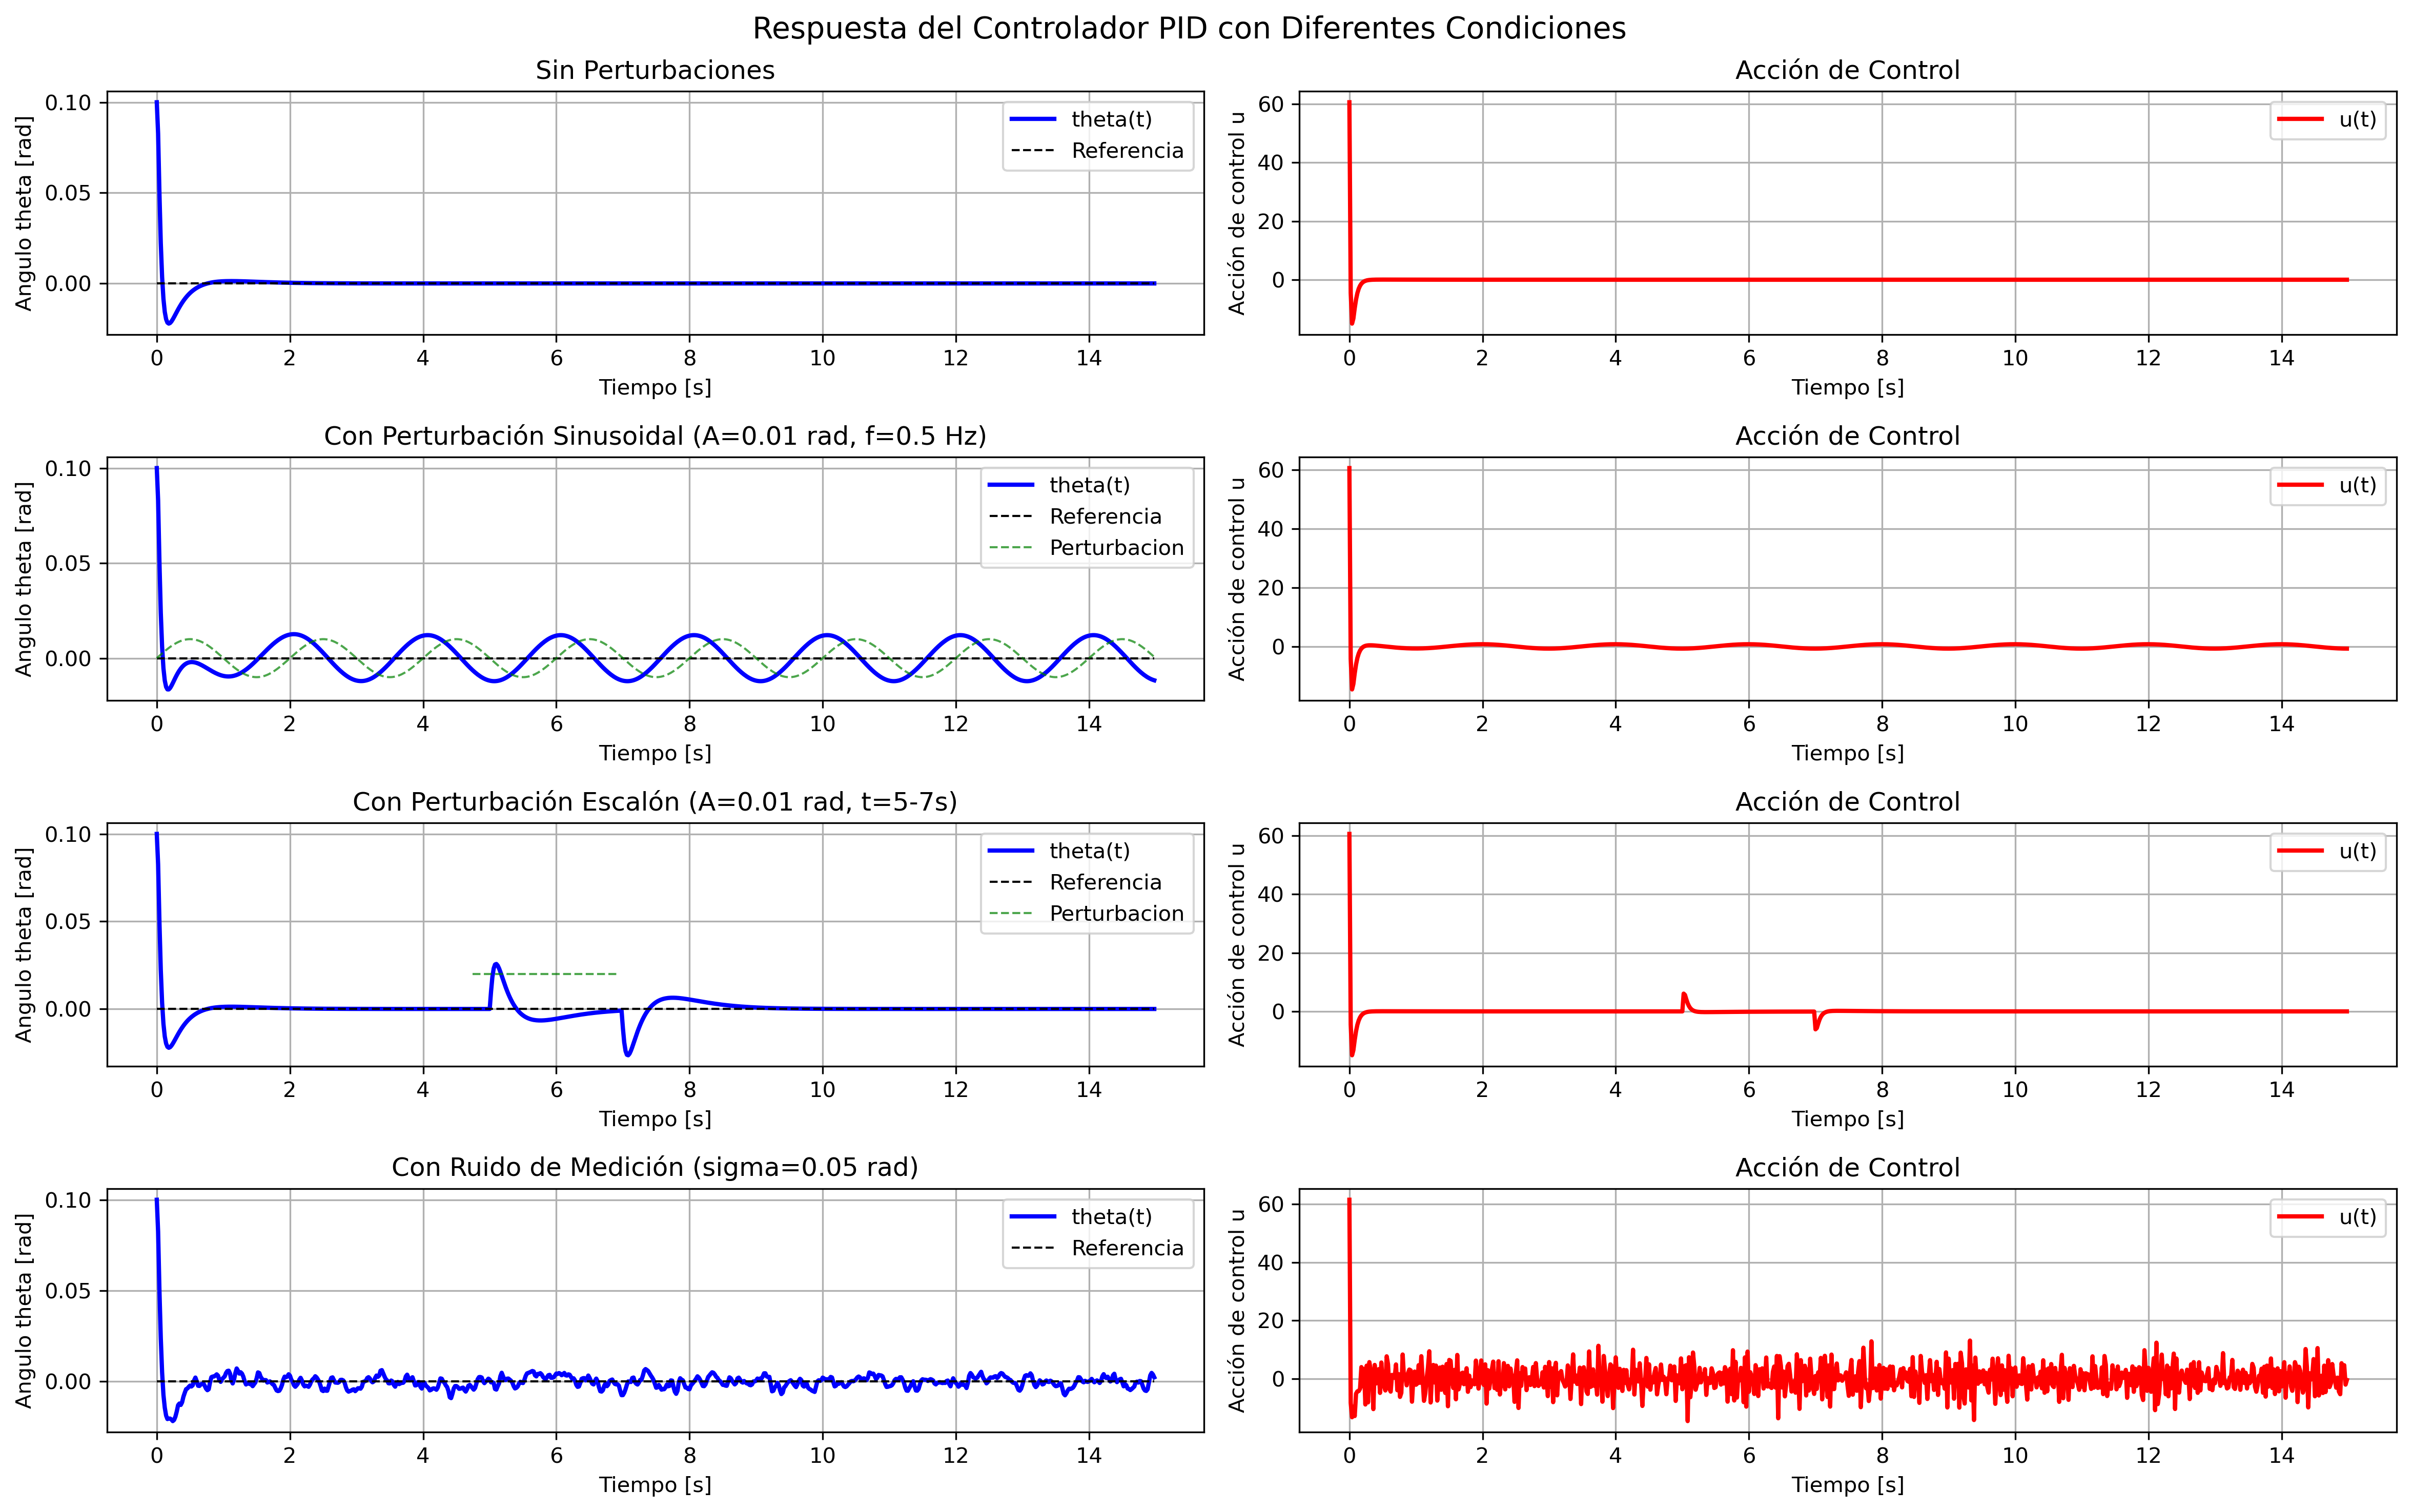
\includegraphics[width=\textwidth]{imagenes_pid/respuesta_pid_condicion_inicial.png}
\end{center}
\end{frame}

\begin{frame}{Análisis de Estabilidad}
\begin{block}{Análisis en el Plano Z}
El sistema discretizado presenta:
\begin{itemize}
\item Polo inestable: $z = 1.083$ ($|z| > 1$)
\item Polo estable: $z = 0.924$ ($|z| < 1$)
\item Cero: $z = -1.0$
\end{itemize}
\end{block}

\begin{block}{Efecto del Controlador PID}
El controlador PID estabiliza el sistema moviendo los polos dentro del círculo unitario ($|z| < 1$), logrando una dinámica controlada deseada.
\end{block}
\end{frame}

\begin{frame}{Mapa de Polos y Ceros}
\begin{center}
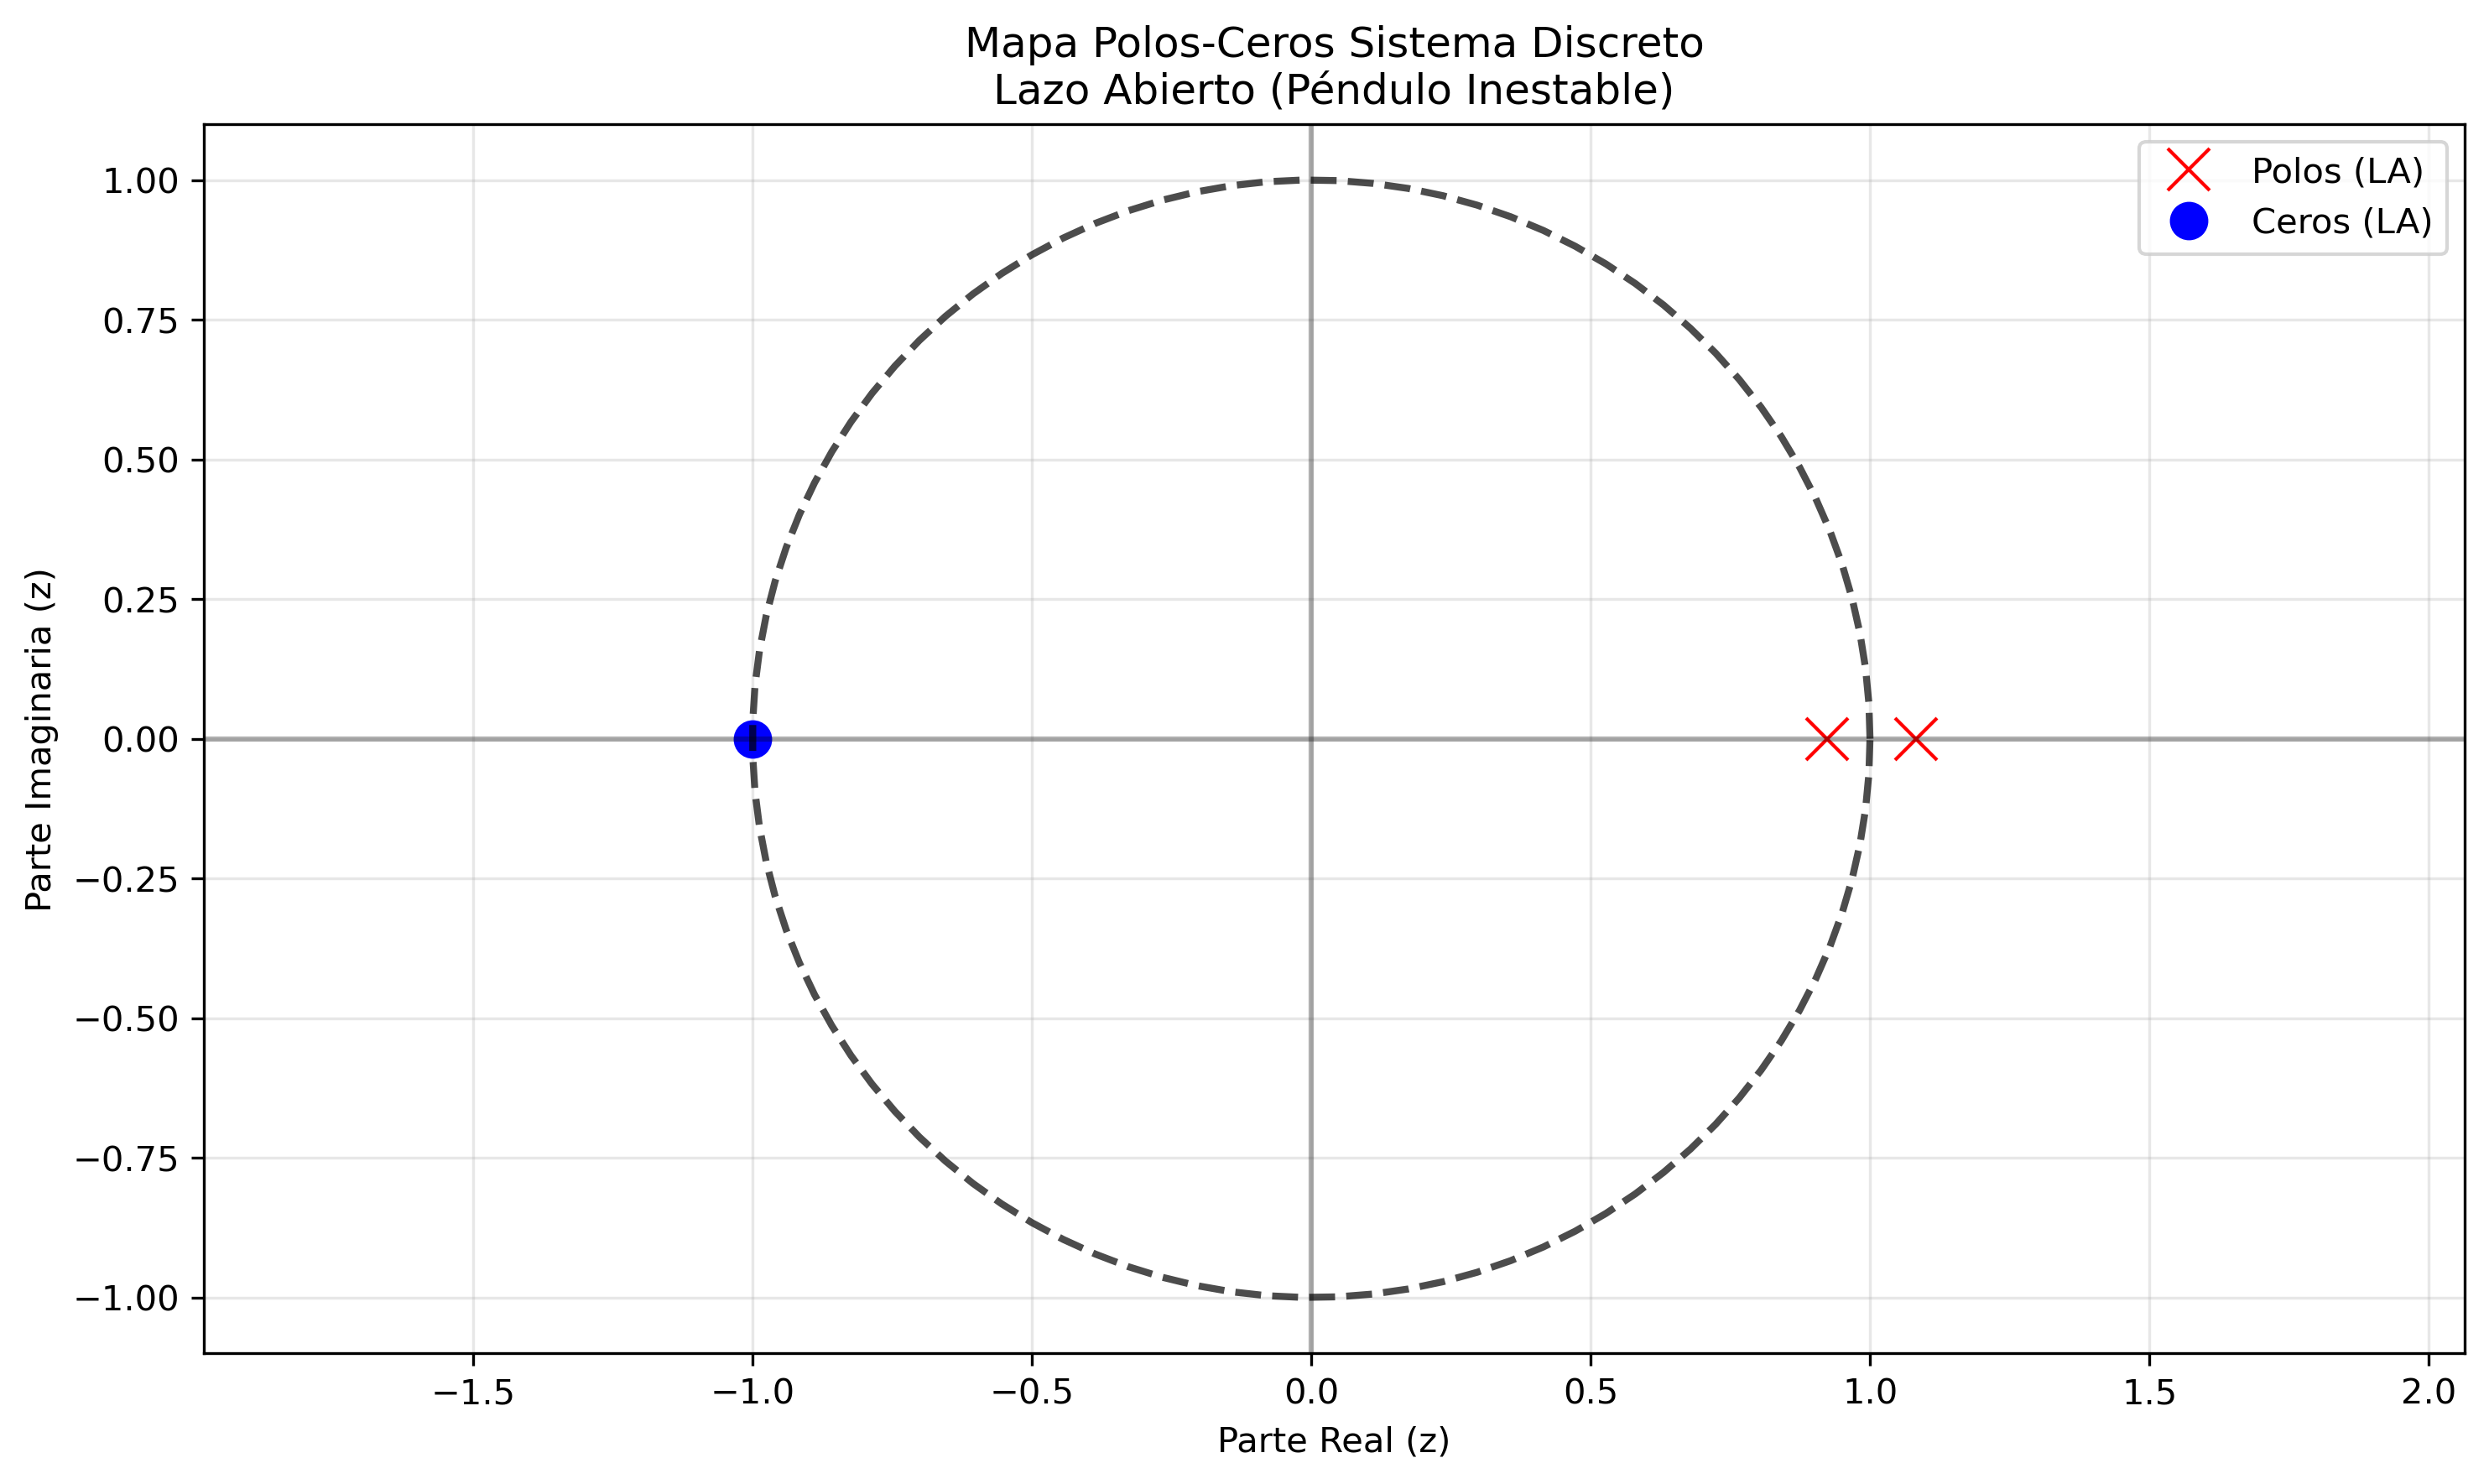
\includegraphics[width=0.8\textwidth]{imagenes_pid/polos_ceros_comparacion.png}
\end{center}

\begin{itemize}
\item Polos del sistema en lazo abierto marcados en rojo
\item Círculo unitario representa la frontera de estabilidad
\item El controlador PID garantiza estabilidad discreta
\end{itemize}
\end{frame}

\begin{frame}{Métricas de Rendimiento}
\begin{block}{Resultados Cuantitativos}
\begin{itemize}
\item Error estacionario: $< 0.001$ rad
\item Tiempo de establecimiento: $\approx 0.08$ s
\item Acción de control máxima: $\approx 60.6$ unidades
\item Estabilidad mantenida en todas las condiciones
\end{itemize}
\end{block}

\begin{block}{Robustez del Sistema}
El controlador demuestra robustez ante:
\begin{itemize}
\item Condiciones iniciales no nulas
\item Perturbaciones sinusoidales
\item Perturbaciones tipo escalón
\item Ruido de medición gaussiano
\end{itemize}
\end{block}
\end{frame}

\section{Sintonización Automática (Autotuning)}

\begin{frame}{Estrategia de Autotuning}
\begin{block}{Metodología en Lazo Cerrado}
Se implementó un mecanismo de auto-ajuste que opera mientras el sistema está en control:
\begin{enumerate}
    \item \textbf{Inicio:} Controlador PID con ganancias conservadoras (baja agresividad).
    \item \textbf{Identificación Online:} Estimación recursiva (RLS) de los parámetros del modelo ARX ($a_1, a_2, b_1, b_2$).
    \item \textbf{Evento de Ajuste ($t=4$s):}
    \begin{itemize}
        \item Conversión del modelo discreto identificado a continuo $G(s)$ (Tustin).
        \item Recálculo de ganancias PID usando Asignación de Polos.
        \item Actualización instantánea del controlador.
    \end{itemize}
\end{enumerate}
\end{block}
\end{frame}

\begin{frame}{Resultados: Autotuning sin Perturbaciones}
\begin{center}
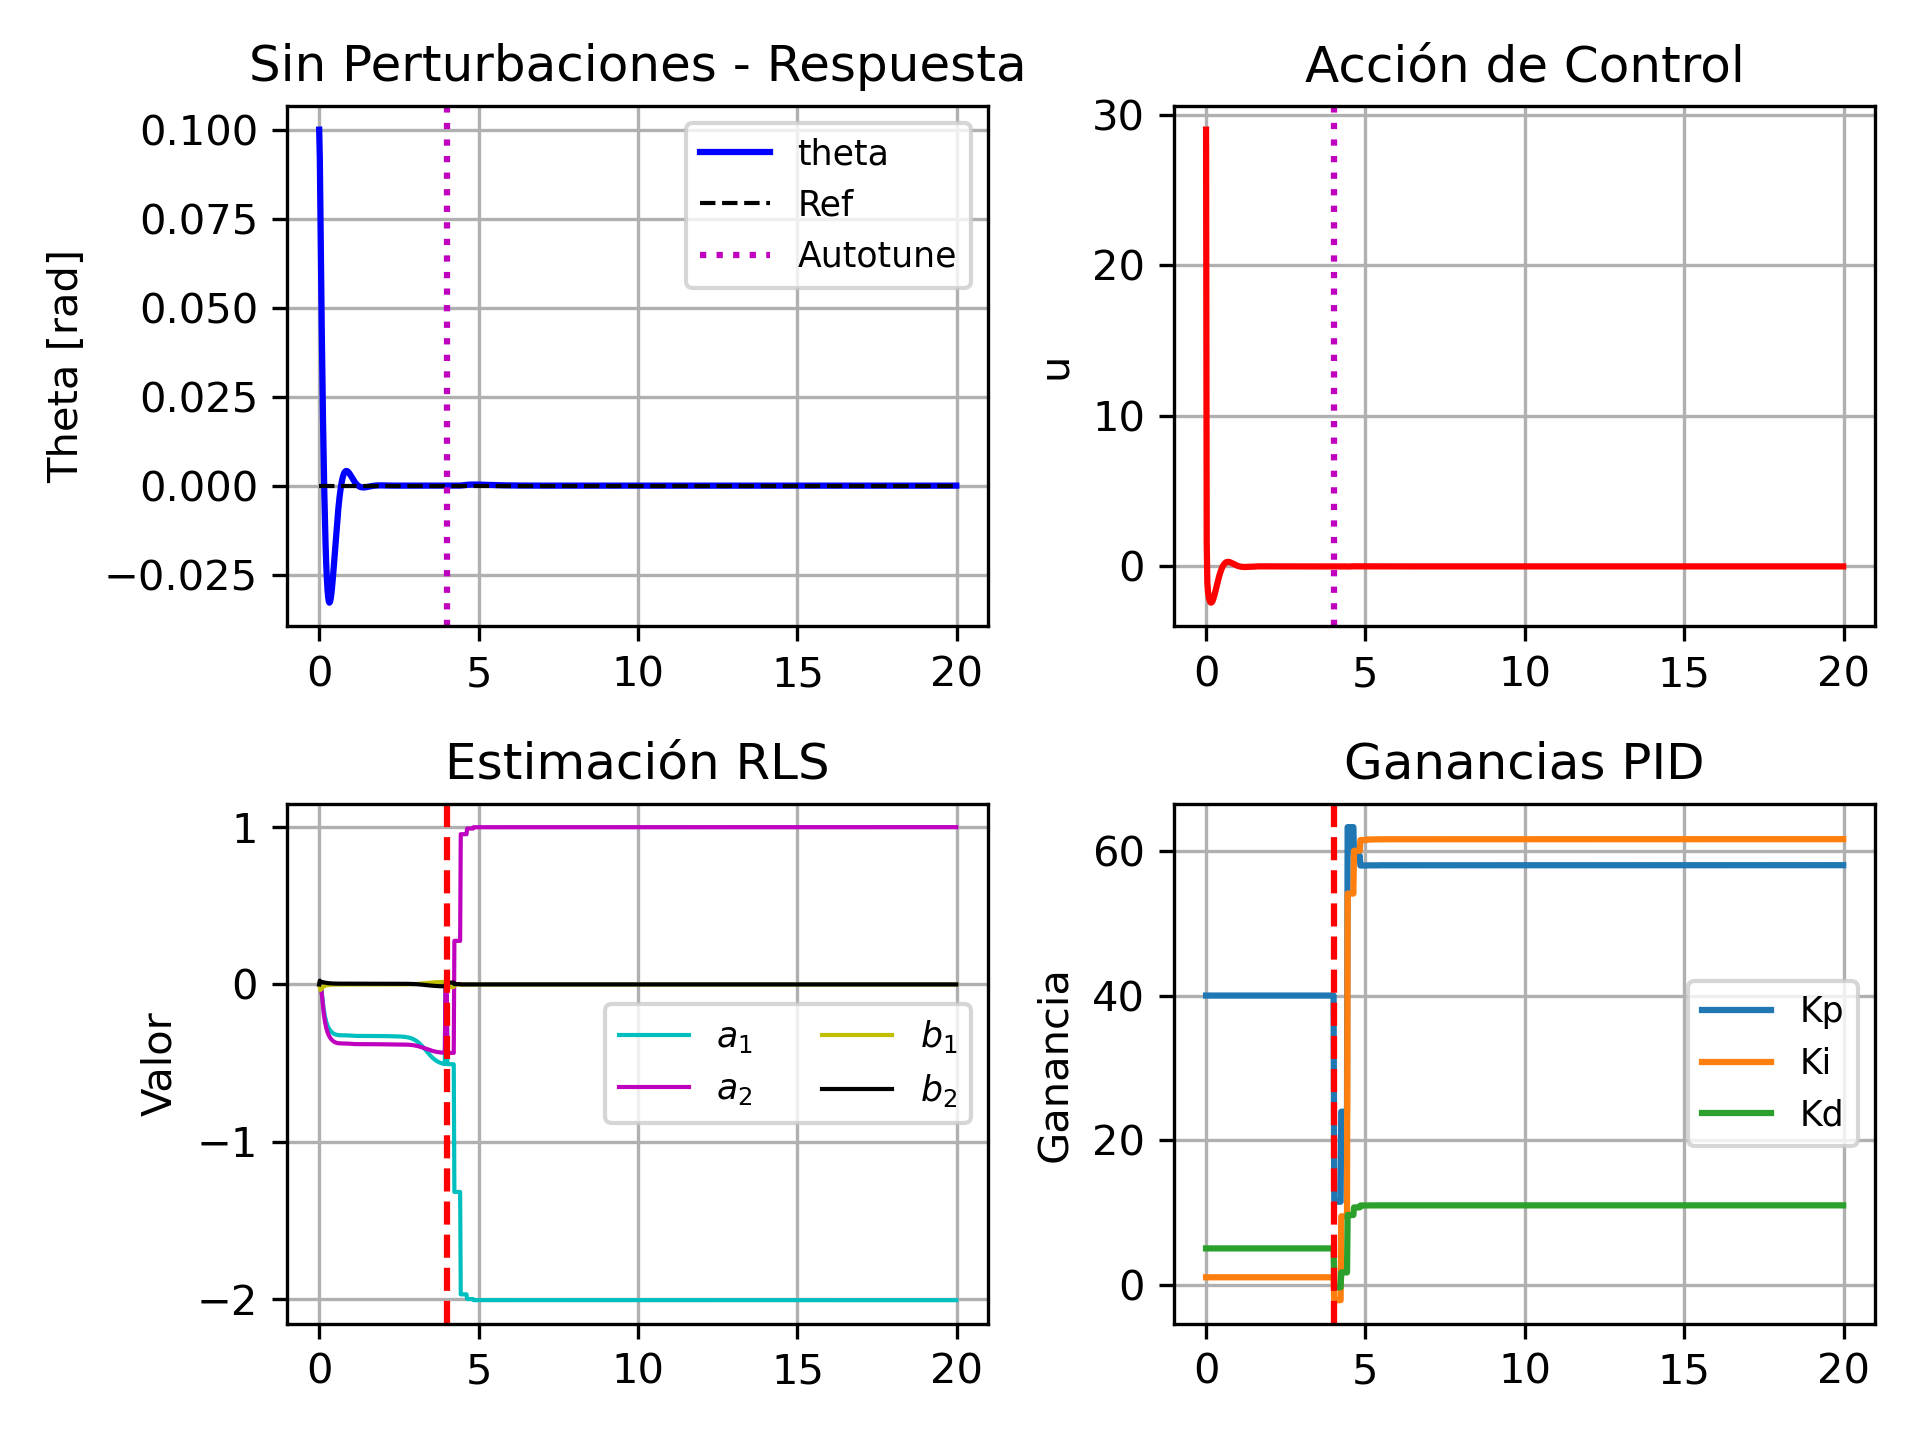
\includegraphics[width=0.9\textwidth]{imagenes_pid_autotunning/autotuning_sin_perturbaciones.png}
\end{center}
\begin{itemize}
    \item En $t=4$s, se observa la actualización de las ganancias PID (gráfico inferior derecho).
    \item La estimación de parámetros converge antes del evento de sintonización.
\end{itemize}
\end{frame}

\begin{frame}{Resultados: Robustez ante Perturbación Sinusoidal}
\begin{center}
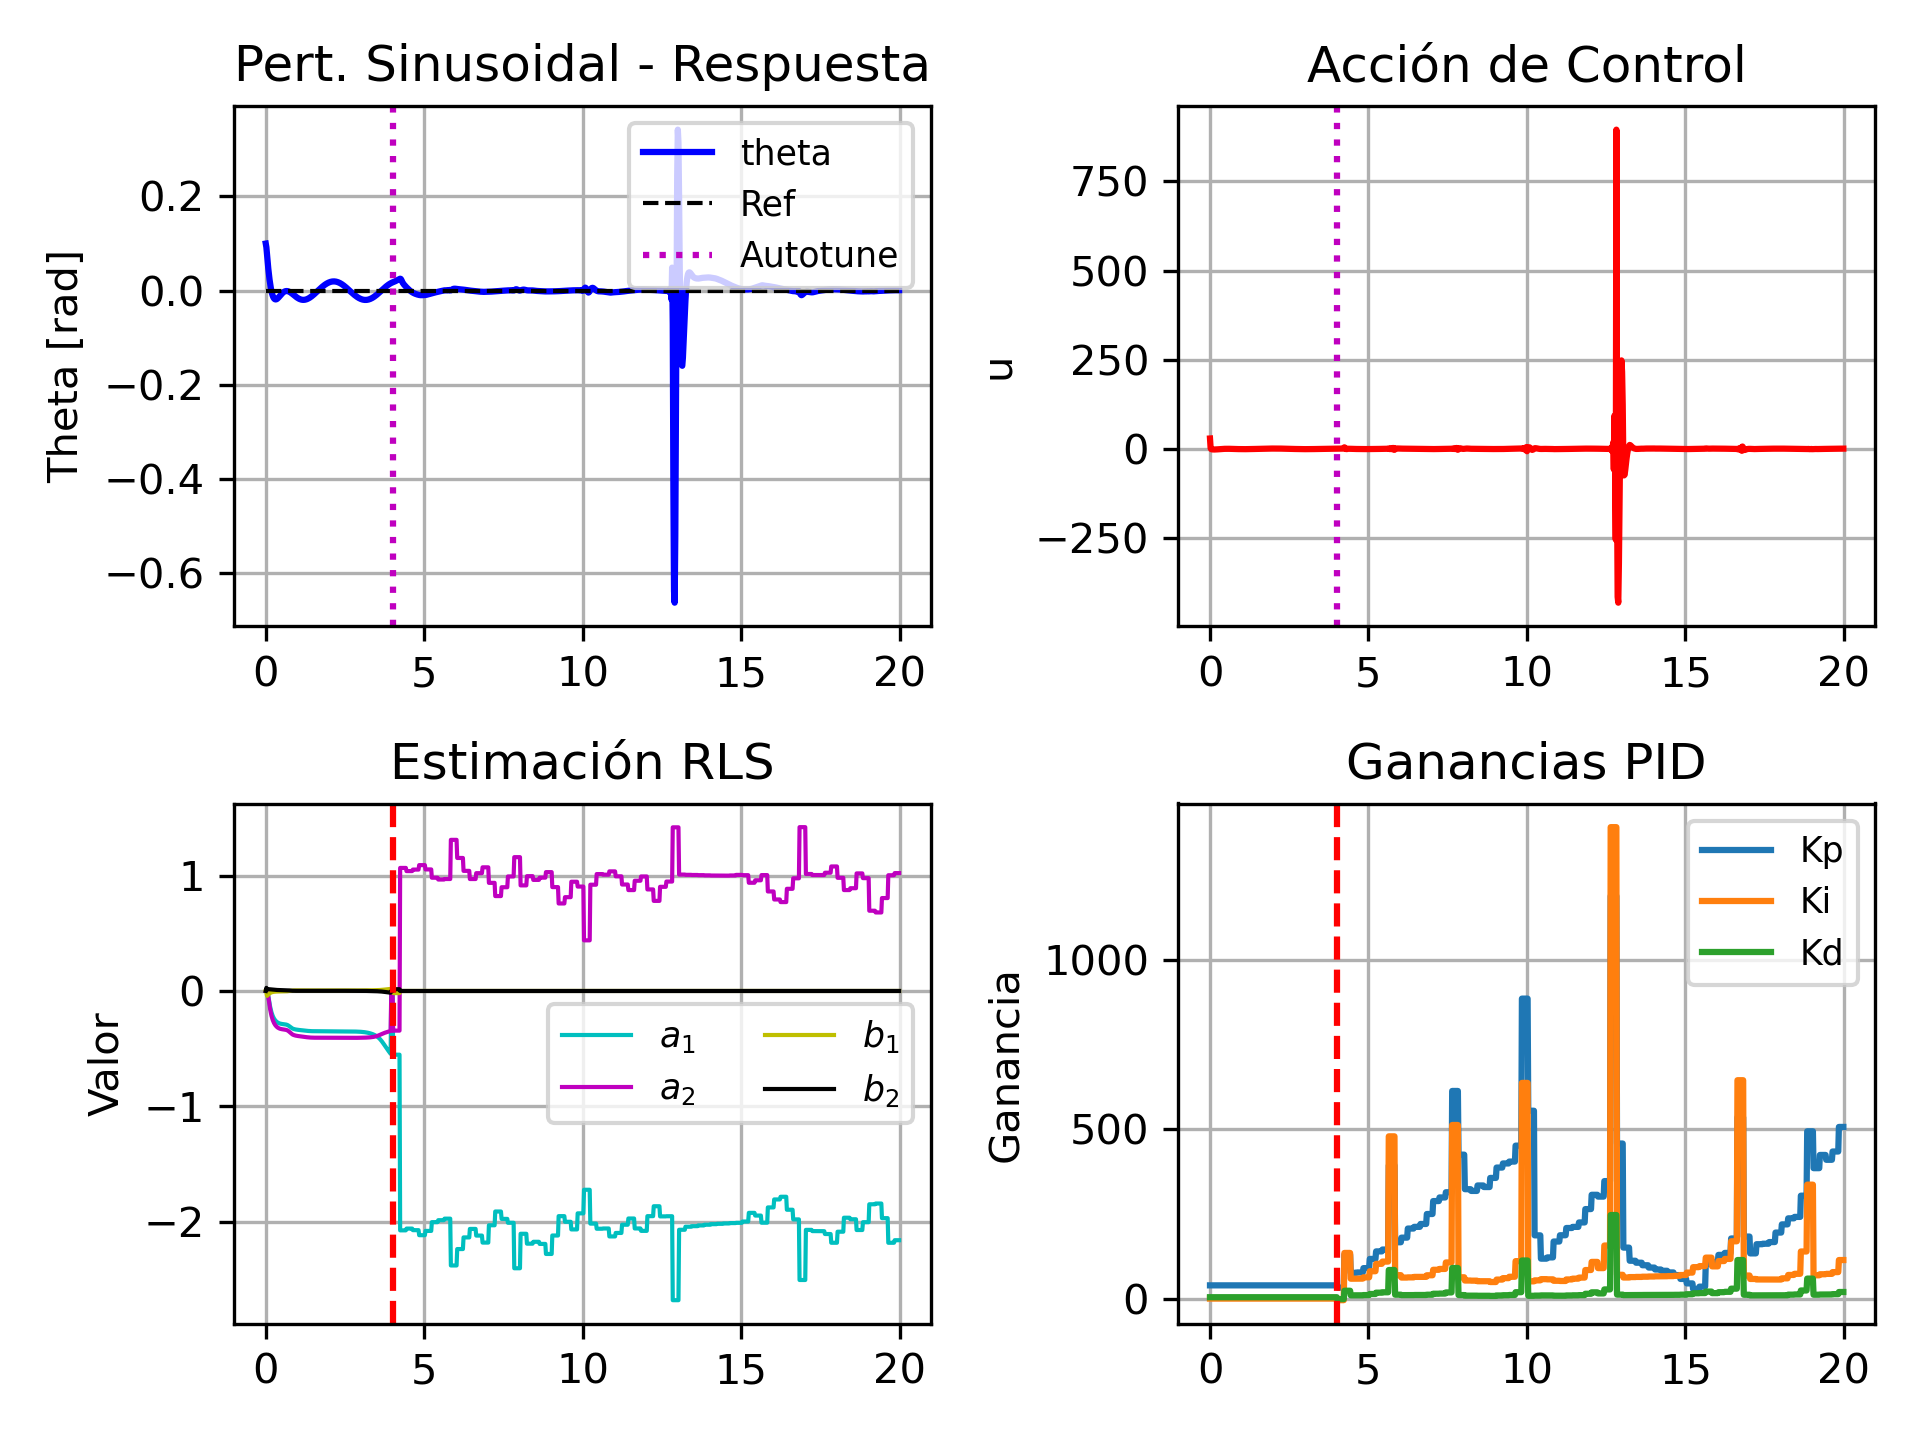
\includegraphics[width=0.85\textwidth]{imagenes_pid_autotunning/autotuning_sinusoidal.png}
\end{center}
\begin{block}{Análisis}
El autotuning ajusta las ganancias para mantener la estabilidad y minimizar el error de seguimiento incluso con una perturbación periódica continua.
\end{block}
\end{frame}

\begin{frame}{Resultados: Robustez ante Perturbación Escalón}
\begin{center}
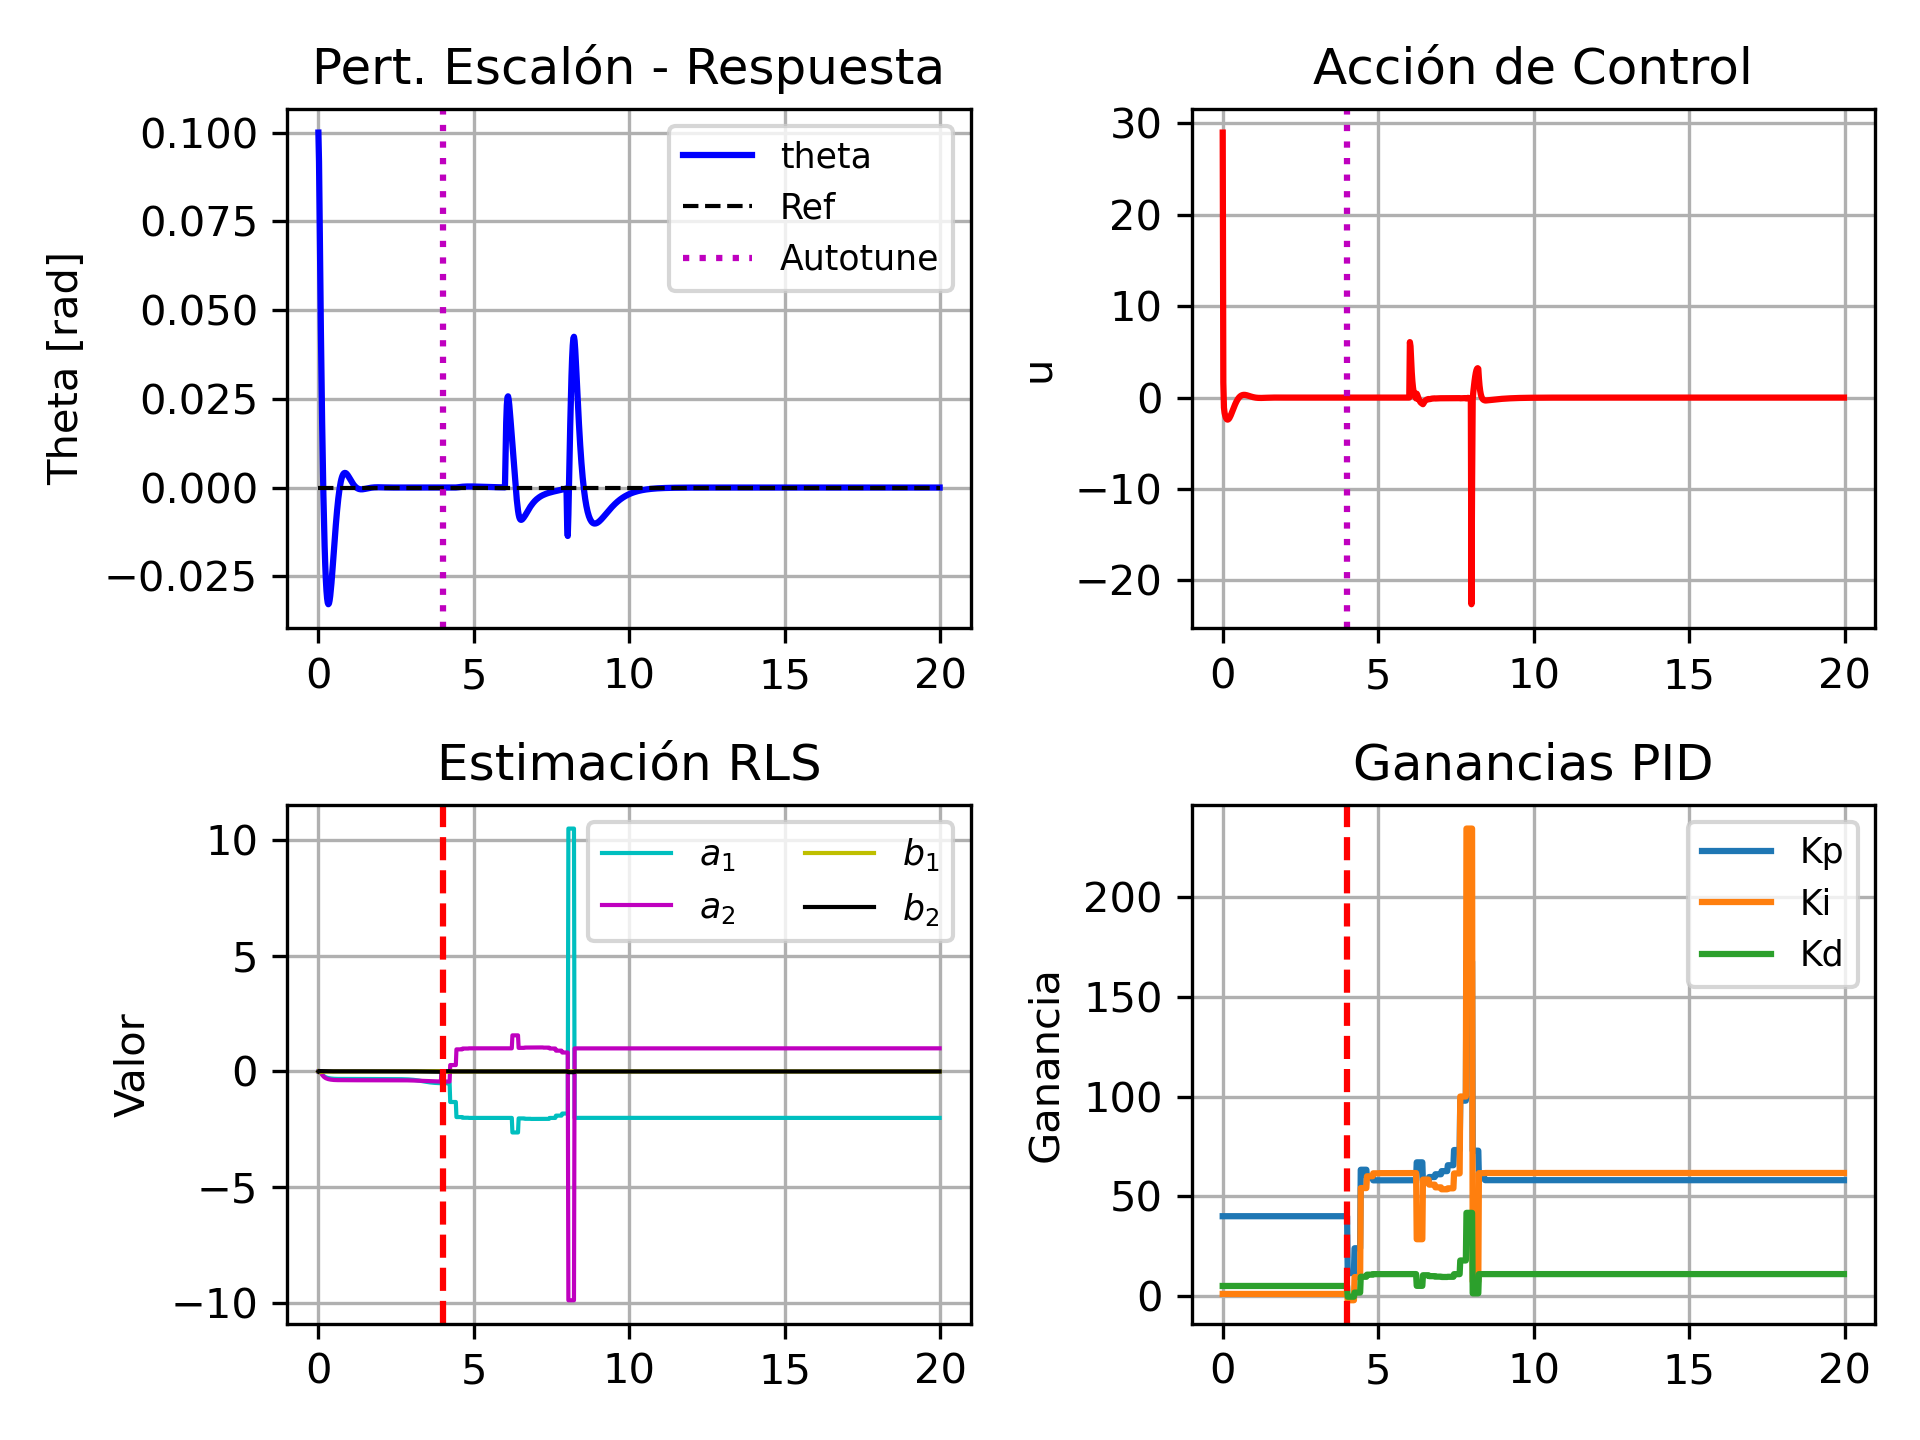
\includegraphics[width=0.85\textwidth]{imagenes_pid_autotunning/autotuning_escalon.png}
\end{center}
\begin{block}{Análisis}
Ante un cambio brusco en la carga (escalón), el controlador re-sintonizado muestra una recuperación rápida y estable.
\end{block}
\end{frame}



\begin{frame}{Resultados: Robustez ante Ruido}
\begin{center}
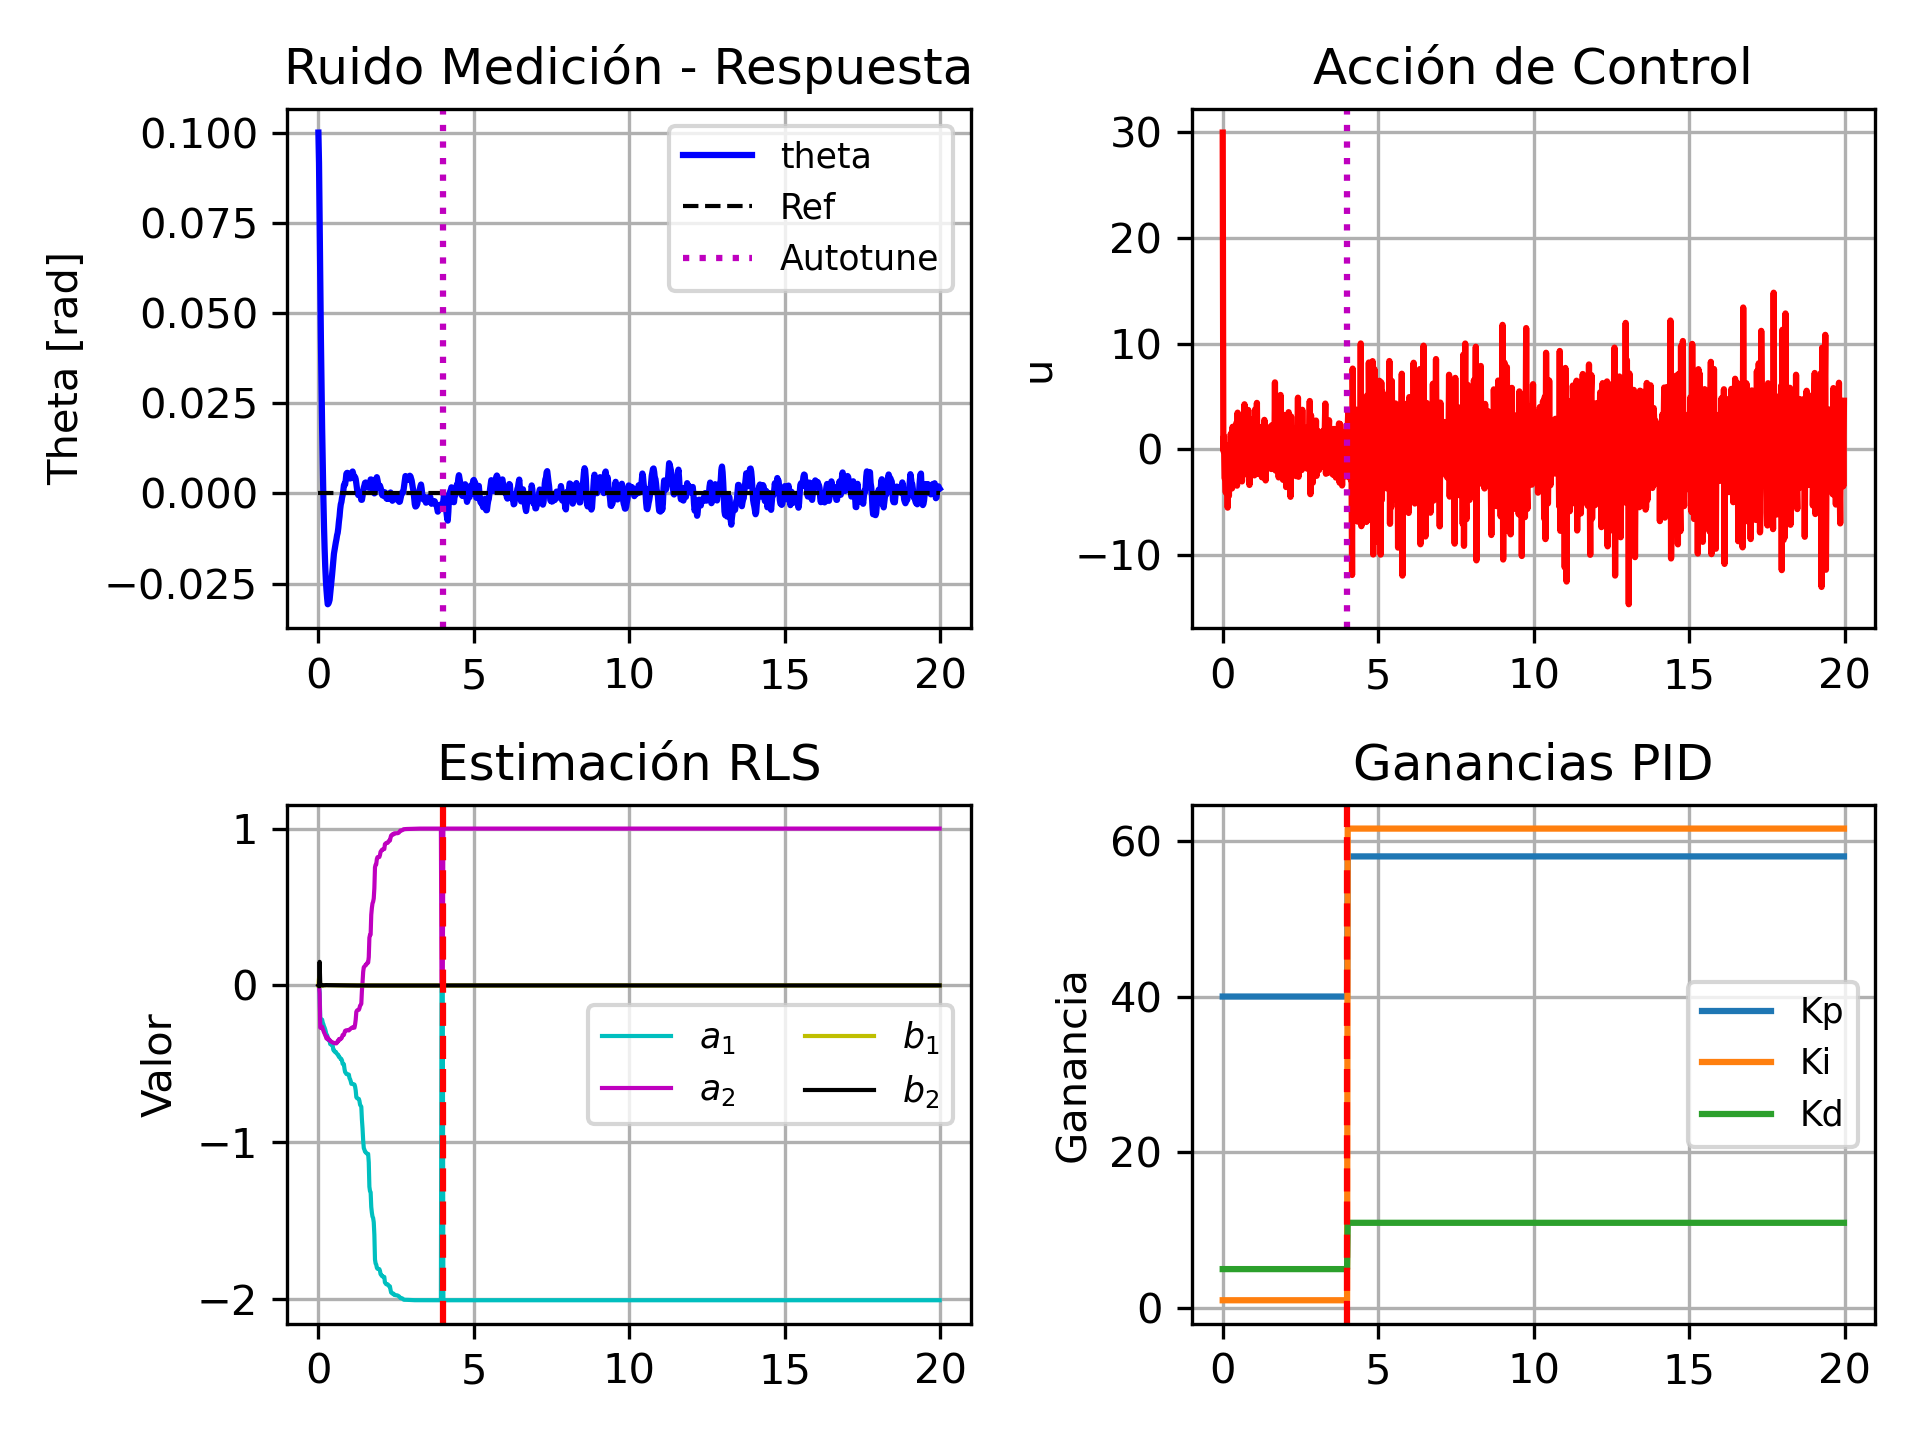
\includegraphics[width=0.8\textwidth]{imagenes_pid_autotunning/autotuning_ruido.png}
\end{center}
\begin{itemize}
    \item El estimador RLS filtra efectivamente el ruido de medición ($\sigma=0.005$).
    \item Los parámetros estimados convergen a pesar del ruido, permitiendo un cálculo válido del PID.
\end{itemize}
\end{frame}

\section{Conclusiones}



\end{document}
